\subsection{SGLang Framework}
{{\footnotesize
\noindent A high-performance open-source serving framework combining efficient backend runtime (RadixAttention, batching, quantization) and expressive frontend language, boosting LLM/VLM inference throughput up to \textasciitilde{}3x over alternatives. 


\begin{description}[labelwidth=4cm, labelsep=1em, leftmargin=4cm, itemsep=0.1em, parsep=0em]
  \item[date:] 2023-12-12
  \item[version:] v0.4.9
  \item[last\_updated:] 2025-06
  \item[expired:] unknown
  \item[valid:] yes
  \item[valid\_date:] 2023-12-12
  \item[url:] \href{https://github.com/sgl-project/sglang/tree/main/benchmark}{https://github.com/sgl-project/sglang/tree/main/benchmark}
  \item[doi:] 10.48550/arXiv.2312.07104
  \item[domain:] LLM Vision
  \item[focus:] Fast serving framework for LLMs and vision-language models
  \item[keywords:]
    - LLM serving
    - vision-language
    - RadixAttention
    - performance
    - JSON decoding
  \item[licensing:] Apache License 2.0
  \item[task\_types:]
    - Model serving framework
  \item[ai\_capability\_measured:]
    - Serving throughput
    - JSON/task-specific latency
  \item[metrics:]
    - Tokens/sec
    - Time-to-first-token
    - Throughput gain vs baseline
  \item[models:]
    - LLaVA
    - DeepSeek
    - Llama
  \item[ml\_motif:]
    - LLM Vision
  \item[type:] Framework
  \item[ml\_task:]
    - Model serving
  \item[solutions:] Solution details are described in the referenced paper or repository.
  \item[notes:] Deployed in production (xAI, NVIDIA, Google Cloud); v0.4.8 release June 2025. 

  \item[contact.name:] SGLang Team
  \item[contact.email:] unknown
  \item[datasets.links.name:] Benchmark configs
  \item[results.links.name:] ChatGPT LLM
  \item[fair.reproducible:] Yes
  \item[fair.benchmark\_ready:] Yes
  \item[id:] sglang\_framework
  \item[Citations:] \cite{zheng2024sglangefficientexecutionstructured}
\end{description}

{\bf Ratings:} ~ \\

\begin{tabular}{p{0.15\textwidth} p{0.07\textwidth} p{0.7\textwidth}}
\hline
Rating & Value & Reason \\
\hline
dataset & 2 & Does not introduce new datasets; instead, it evaluates performance using existing model benchmarks.
Only configuration files are included.
 \\
documentation & 4 & Strong GitHub documentation, install guides, and benchmarks. Some advanced topics (e.g.,
scaling, hardware tuning) could use deeper walkthroughs.
 \\
metrics & 5 & Serving-related metrics such as tokens/sec, time-to-first-token, and throughput gain vs. baselines
are well-defined and consistently applied.
 \\
reference\_solution & 3 & Provides benchmark configs and example integrations (e.g., with LLaVA, DeepSeek), but not all
models or scripts are runnable out-of-the-box.
 \\
software & 5 & Actively maintained and production-deployed (e.g., xAI, NVIDIA); source code available under
Apache 2.0. Includes efficient backends (RadixAttention, quantization, batching) and full
serving infrastructure.
 \\
specification & 4 & The framework clearly defines performance targets, serving logic, and model integration.
Input/output expectations are consistent, but not all benchmarks are standardized.
 \\
\hline
\end{tabular}

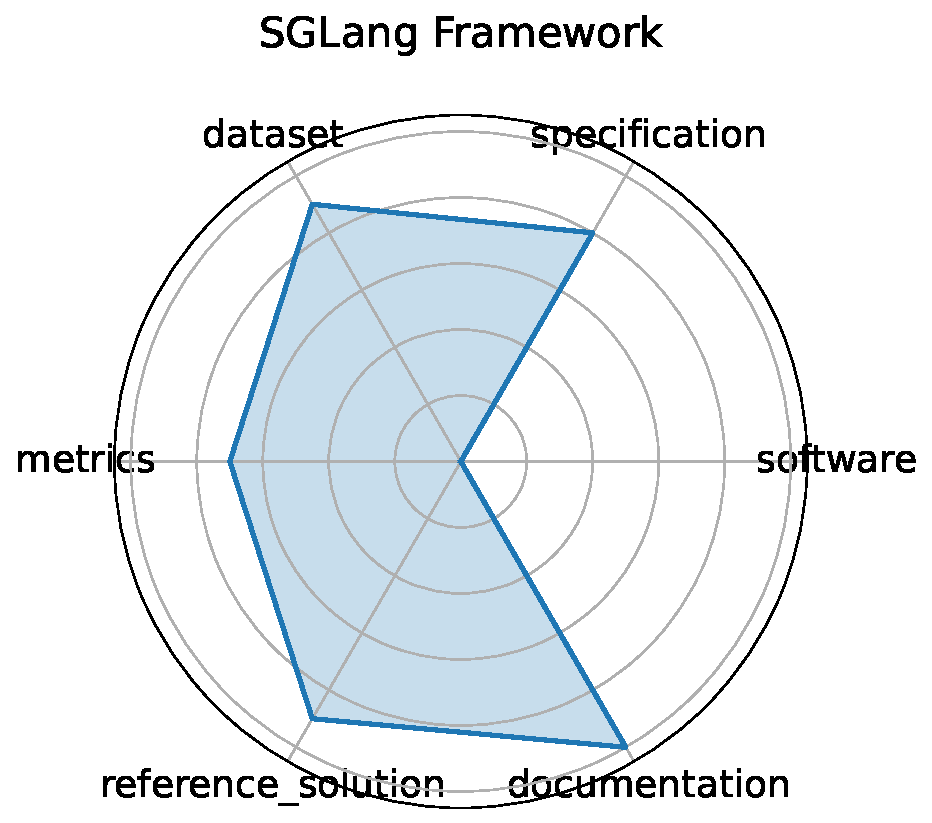
\includegraphics[width=0.2\textwidth]{sglang_framework_radar.pdf}
}}
\clearpage